\begin{samplecase}
{\bf Coupled-channels vibrational model: n + ${}^{74}$Ge}\newline

In this sample case we consider a neutron-induced reaction on
the vibrational nucleus $^{74}$Ge which consists of a 
one-phonon state ($2^{+}$) followed by a $(0^{+}, 2^{+}, 4^{+})$ triplet of 
two-phonon states, and a $3^{-}$ phonon state. The coupling scheme as stored in 
{\em structure/deformation/exp/z032} is automatically adopted. The following 
input file is used:

\VerbatimInput{\samples n-Ge074-vib/org/talys.inp}

In Fig.~\ref{geinel}, the calculated inelastic scattering to the first 
discrete state is plotted.
\end{samplecase}
\begin{figure}
\centering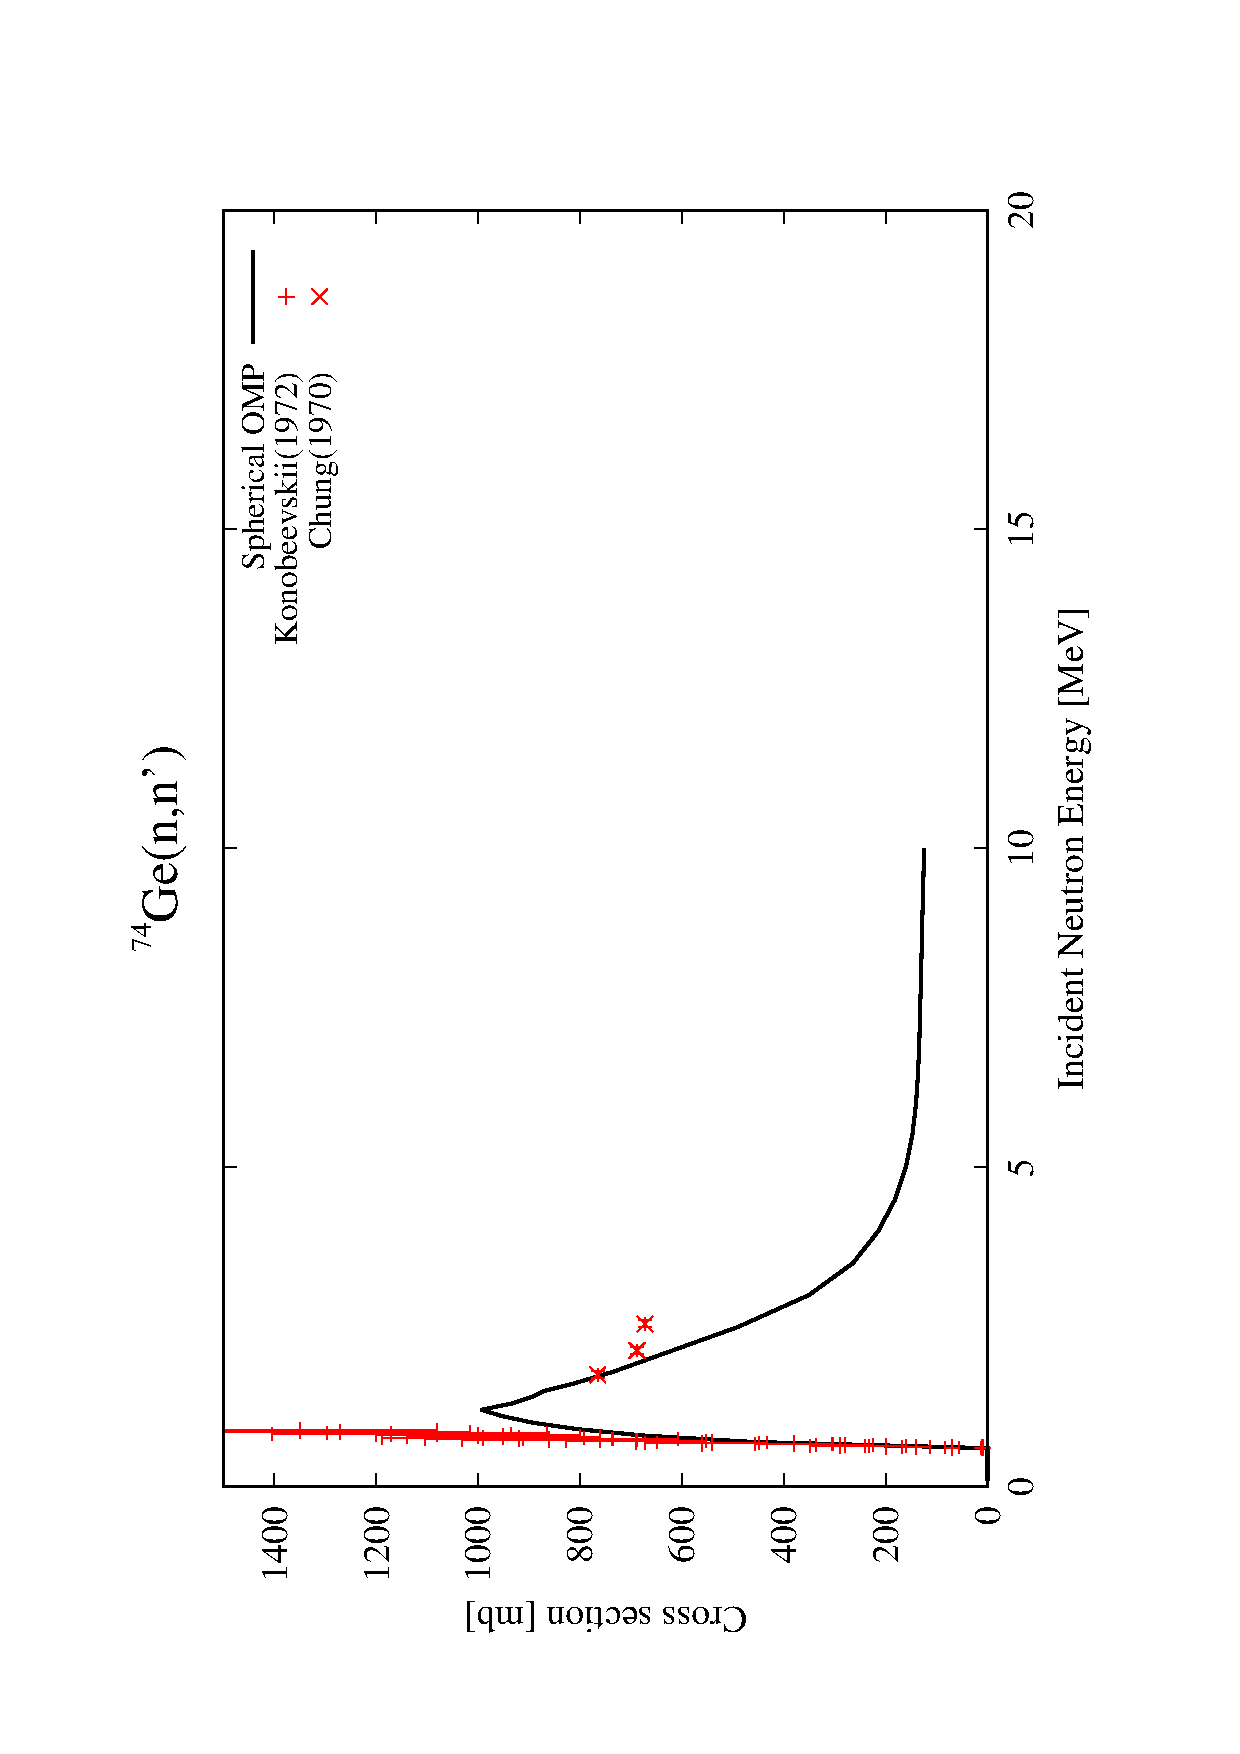
\includegraphics[scale=0.5,angle=270]{n-Ge074-inel}
\caption{Inelastic scattering to the first discrete state of ${}^{74}$Ge.}
\label{geinel}
\end{figure}
